\documentclass[12pt]{article}   	% use "amsart" instead of "article" for AMSLaTeX format
\usepackage[margin=1in]{geometry}                		% See geometry.pdf to learn the layout options. There are lots.
\geometry{letterpaper}                   		% ... or a4paper or a5paper or ... 
%\geometry{landscape}                		% Activate for for rotated page geometry
\usepackage[parfill]{parskip}    		% Activate to begin paragraphs with an empty line rather than an indent
\usepackage{graphicx}				% Use pdf, png, jpg, or eps§ with pdflatex; use eps in DVI mode
								% TeX will automatically convert eps --> pdf in pdflatex	
\graphicspath{ {images/} }
\usepackage{amsmath}
\usepackage{amssymb}
\usepackage{bm}
\usepackage{amsthm}
\usepackage{mathrsfs}
\usepackage{amsbsy}
\usepackage{braket}
\usepackage{enumitem}
\usepackage{listings}
\usepackage{dsfont}
\usepackage [english]{babel}
\usepackage [autostyle, english = american]{csquotes}
\MakeOuterQuote{"}
\newcommand\p[2]{\dfrac{\partial #1}{\partial #2}}
\newcommand\der[2]{\dfrac{d #1}{d #2}}
\title{Computational Physics\\Final Project}
\author{Mukesh Ghimire}
\date{}							% Activate to display a given date or no date

\begin{document}
\maketitle
\begin{abstract}
	This paper summarizes a particle mesh simulation of the evolution of large-scale structure of dark 
	matter. The simulation uses gaussian random fields and FFTs to produce initial conditions at 
	redshift 50 from a power spectrum, cloud-in-cell interpolation to map particles' masses onto grid 
	points to find density fluctuations, FFTs to solve a Poisson equation for gravitational potential, 
	cloud-in-cell interpolation to map forces from grid points onto the particles, and a Runge-Kutta 
	solver of order 4 to evolve the particles in time. The scale factor of the universe is used instead of 
	time as the evolution parameter, and it is evolved to modern day. A power spectrum is then 
	produced from the results and compared to the Zel'dovich approximation as well as the original 
	power spectrum used to set the initial conditions.
\end{abstract}

\section*{Introduction}
The large scale structure in the universe today is postulated to be due to perturbations in the 
homogeneous and smooth early universe predicted by inflation. Various cosmological models and
theories make predictions for these perturbations, and simulations are an important tool to extrapolate
them to observable predictions.

Cosmological models predict power spectra, which describe the density fluctuations in the universe.
These fluctuations can be produced by taking a complex random Gaussian field at three dimensional
Fourier modes and scaling it with respect to the power at the modulus of the mode:
\begin{equation}
	\delta(\vec k) = \sqrt{\frac{P(|\vec k|)}{2}}(\text{gauss}(0,1) + i\ \text{gauss}(0,1))
\end{equation}
The gradient of this average fluctuation field can then be inverse Fourier transformed to perturb 
particles on a $N^3$ grid:
\begin{align}
	\vec \psi(\vec k) &= -i\vec k \delta(\vec k)\\
	\vec\psi(\vec k) &\overset{\text{IFFT}}{\to}\vec \psi(\vec x) \nonumber \\
	\vec x_{\text{perturbed}} &= \vec x_{\text{grid}} + D_+(t)\vec \psi(\vec x)
\end{align}
where $D_+(t)$ is called the linear growth function and has a value of $0.0257$ at redshift 50, which
is where the data is initialized.

Equation (3) is called the Zel'dovich approximation. It is a good approximation for the positions of
particles in the early universe (40-70 redshift), but it gets worse because it is a linear approximation.
It does not account for gravity, so in the long run the particles in its model overshoot their true
trajectories, as they keep traveling in straight lines at constant speed and don't clump with other
particles. However, the Zel'dovich approximation can be used to get a good idea for the general
motion of particles.

These conditions calculated by (3) are then evolved using the equation
\begin{equation}
	\der{^2\vec x}{\tau^2} + \frac{a'}{a}\der{\vec x}{\tau} = - \nabla\phi(\vec x)
\end{equation}
where $a$ is the scale factor of the universe, $\tau$ is conformal time, and $\phi$ is the gravitational
potential.

This differential equation can be rewritten to have $a$ as the evolving parameter, because it is
much easier to work with $a$ in cosmology than it is with conventional units of time.
\begin{equation}
	\der{^2\vec x}{a^2} + \frac{3}{2a}\left[\frac{\Omega_{de}a^3}
	{\Omega_m+\Omega_{de}a^3}+1\right]\der{\vec x}{a} =  -\frac{\nabla\phi(\vec x)}{a'^2}\\
\end{equation}
However, in order to numerically solve this differential equation, $\phi(\vec x)$ needs to be evaluated at
each time step via the Poisson equation
\begin{equation}
	\nabla^2\phi = 4\pi G\Omega_m\rho_{\text{crit}}a^{-1}\delta
\end{equation}
where $G$ is the gravitational constant, $\Omega_m$ is the density of matter today in units of critical
density, and $\rho_{\text{crit}}\approx 8.58\times 10^{-18}$kg/km$^3$ is the critical density. $\delta = 
\dfrac{\rho - \bar\rho}{\bar\rho}$ is the fluctuation field, where $\rho$ is the density field and $\bar\rho$ is 
the average density in the box.

The density field at the grid points can be calculated from the positions of the particles by using an
interpolation method. The density field is then used to find the fluctuation field, which can then be 
Fourier transformed  and used to find the gradient of $\phi$ in Fourier space:
\begin{align}
	\delta(\vec x) &= \frac{\rho(\vec x) - \bar\rho}{\bar\rho}\\
	\delta(\vec x) &\overset{\text{IFFT}}{\to} \delta(\vec k) \nonumber \\
	\nabla \phi(\vec k) &= \frac{-i\vec k4\pi G\Omega_m\rho_{\text{crit}}\delta(\vec k)}{a |\vec k|^2}
\end{align}
This can then be inverse Fourier transformed to get $\nabla\phi (\vec x)$ at the grid points. However 
these forces need to be assigned to the particles, which will most likely not be at the grid points at 
future time steps in the evolution. This is done by using a reverse of the interpolation method used
to find the density field.

The final piece of the puzzle in equation (5) is $a'$, which is given by
\begin{align*}
	a' = \sqrt{\frac{8\pi G\rho_{\text{crit}}}{3}(\Omega_ma+\Omega_{de}a^4)}
\end{align*}
where $\Omega_{de}$ is the density of dark energy today in units of $\rho_{\text{crit}}$.

With these functions and parameters, the equation of motion is complete, and can be solved to find
the time-evolution of the system.

The final state of particles can be used to produce a power spectrum. This is done by creating a
fluctuation field $\delta$ as in equation (7), finding its Fourier transform, and using the formula:
\begin{equation}
	P(k) = \frac{1}{N_{k\text{-shell}}}\sum_{\vec q\in k\text{-shell}}|\delta(\vec q)|^2
\end{equation}
where $k$-shell is a shell with variable thickness centered at the sphere of radius $k$ and
$N_{k\text{-shell}}$ is the number of particles in this shell.

This power spectrum can be compared to the spectrum used to set up the initial conditions to check
the accuracy of the simulation.

\section*{Methodology}

A particle mesh of a million points ($100\times100\times100$) was simulated in a box of side $100$ 
Mpc/h. Periodic boundary conditions were used to ensure an approximately homogeneous and isotropic 
simulated universe and to contain the particles inside the box for a stable simulation. \texttt{numpy} 
arrays were used to store the position and velocity information of each particle and to calculate the 
numerous physical quantities mentioned in the previous section.

The initial conditions were set using a power spectrum for redshift 0, but multiplied by $D+^2$ at
redshift 50 to scale it back in time. The initial positions were plotted to get a general idea of the 
perturbations.

The equations in the previous section were programmed and solved using mostly \texttt{numpy} 
functions due to their incredible efficiency. The \texttt{numpy.fft.rfftn} and \texttt{numpy.fft.irfftn} 
functions were used to Fourier transform and inverse Fourier transform the data whenever needed.
\texttt{numpy.random.normal} was used as the gaussian random number generator to create the 
random gaussian field required for the initial conditions. Finally, numerous \texttt{numpy} array functions
were used to expedite computing processes and make the code more efficient overall.

A cloud-in-cell interpolator was programed to calculate the density field at each time step. This is an 
interpolation method that divides the particles into its nearest grid points using its proximity 
to them. These fractions add up to one and are proportional to the distance between the particle and 
the respective grid point.  The cloud-in-cell interpolator was coded using a for loop, since the particles' 
positions were converted to array indices to update the mass contributions at each grid point. For a 
particle with position $(x_p,y_p,z_p)$, its integer floor $(i,j,k)$ was found, which lies at a grid point, and 
fractions were assigned:
\begin{align*}
	d_x = x_p - i,\ & d_y = y_p - j,\ d_z = z_p - k\\
	t_x = 1 - d_x,\ & t_y = 1 - d_y,\ t_z = 1 - d_z
\end{align*}
The fractional divisions were then interpolated using:
\begin{align*}
	\rho_{i,j,k} &= \rho_{i,j,k} + m_pt_xt_yt_z\\
	\rho_{i+1,j,k} &= \rho_{i+1,j,k} + m_pd_xt_yt_z\\
	\rho_{i,j+1,k} &= \rho_{i,j+1,k} + m_pt_xd_yt_z\\
	\rho_{i,j,k+1} &= \rho_{i,j,k+1} + m_pt_xt_yd_z\\
	\rho_{i+1,j+1,k} &= \rho_{i+1,j+1,k} + m_pd_xd_yt_z\\
	\rho_{i,j+1,k+1} &= \rho_{i,j+1,k+1} + m_pt_xd_yd_z\\
	\rho_{i+1,j,k+1} &= \rho_{i+1,j,k+1} + m_pd_xt_yd_z\\
	\rho_{i+1,j+1,k+1} &= \rho_{i+1,j+1,k+1} + m_pd_xd_yd_z
\end{align*}
where $m_p = \dfrac{\bar\rho L^3}{N^3}$ is the mass of each particle in the simulation ($L$ is the grid
size in each dimension).

Reverse cloud-in-cell interpolation is used to assign the calculated forces to the particles. This is done 
with the same $d_{x,y,z}$ and $t_{x,y,z}$ as before, except they are multiplied to the forces from the 
corresponding cells and these products are then summed up to find the total force acting on the 
particle:
\begin{align}
	\vec F_p &= \vec g_{i,j,k}t_xt_yt_z+\vec g_{i+1,j,k}d_xt_yt_z+\vec g_{i,j+1,k}t_xd_yt_z
	+\vec g_{i,j,k+1}t_xt_yd_z \nonumber \\
	&\quad +\vec g_{i+1,j+1,k}d_xd_yt_z+\vec g_{i,j+1,k+1}t_xd_yd_z
	+\vec g_{i+1,j,k+1}d_xt_yd_z+\vec g_{i+1,j+1,k+1}d_xd_yd_z
\end{align}

A Runge-Kutta solver of order 4 is used to solve (5) and evolve the particles in time. This was chosen
due to its fourth order accuracy.

The final results were plotted alongside the Zel'dovich prediction for modern day.

The cloud-in-cell interpolator was used again to find the density fluctuations of the simulation final state 
and the Zel'dovich approximation in order to calculate their power spectra. The power spectra were 
calculated at $k_n = \dfrac{2\pi n}{200}$ for $n = [0,200]\in\mathbb{Z}$.An additional correction
was made to the power spectrum of the simulation final state to account for the shot noise that emerges
from the discrete nature of the simulation:
\[
	P_{\text{corrected}} = P_{\text{simulation}} - \frac{1}{\overline N}\frac{1}{(2\pi)^3}
\]
where $\overline N$ is the average number of particles per unit volume in the simulated box.

The corrected power spectrum and Zel'dovich power spectrum were graphed alongside the original 
power spectrum.
\clearpage

\section*{Results}
\begin{figure}[h!]
\centering
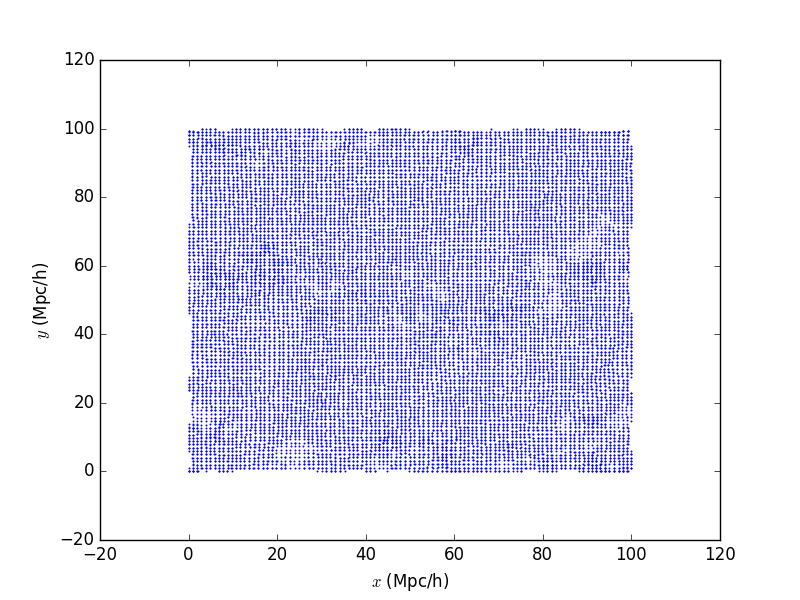
\includegraphics[scale=0.85]{init100.png}
\caption{Graphical representation of top two slices (total of 2 Mpc thickness) of initially perturbed grid
(redshift 50, $a =$ 0.02)}
\end{figure}
\begin{figure}[h!]
\centering
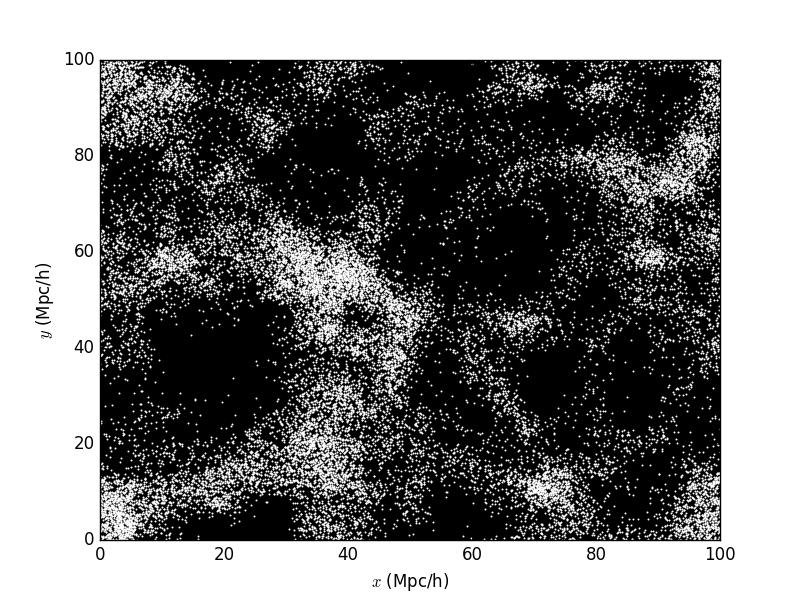
\includegraphics[scale=0.85]{Zeldovich100.png}
\caption{Graphical representation of top two slices (total of 2 Mpc thickness) of Zel'dovich
prediction for modern day (redshift 0, $a =$ 1)}
\end{figure}
\begin{figure}[h!]
\centering
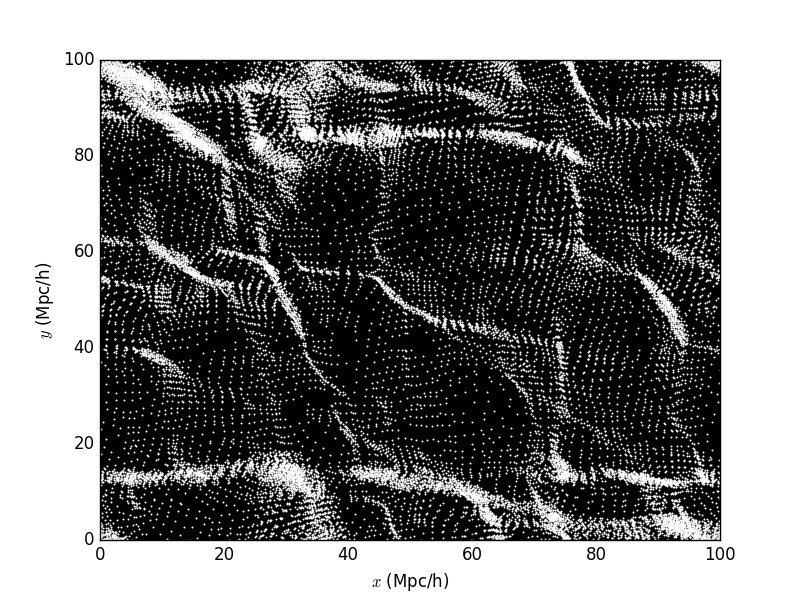
\includegraphics[scale=0.85]{final100.png}
\caption{Graphical representation of top two slices (total of 2 Mpc thickness) of simulation prediction for 
modern day (redshift 0, $a =$ 1)}
\end{figure}
\begin{figure}[h!]
\centering
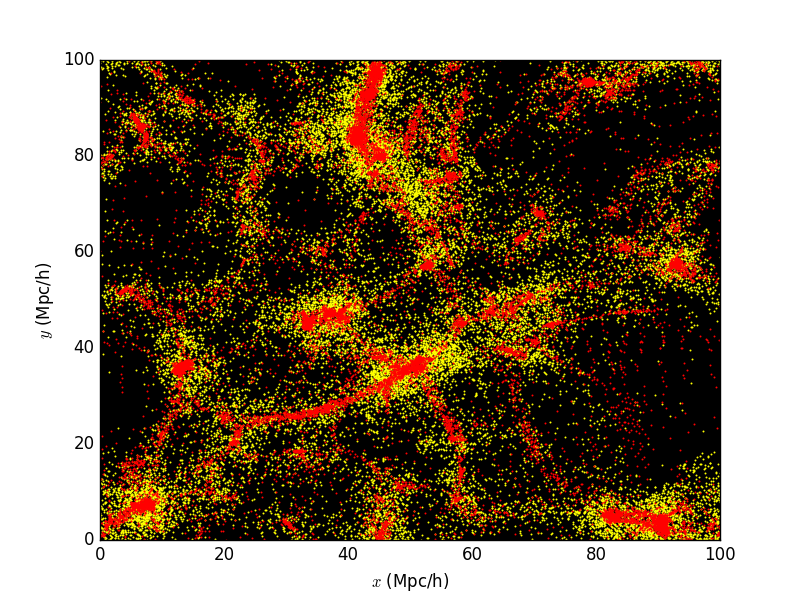
\includegraphics[scale=0.85]{RZoverlap100.png}
\caption{Overlap of Figure 2 (yellow) and 3 (red)}
\end{figure}
\begin{figure}[h!]
\centering
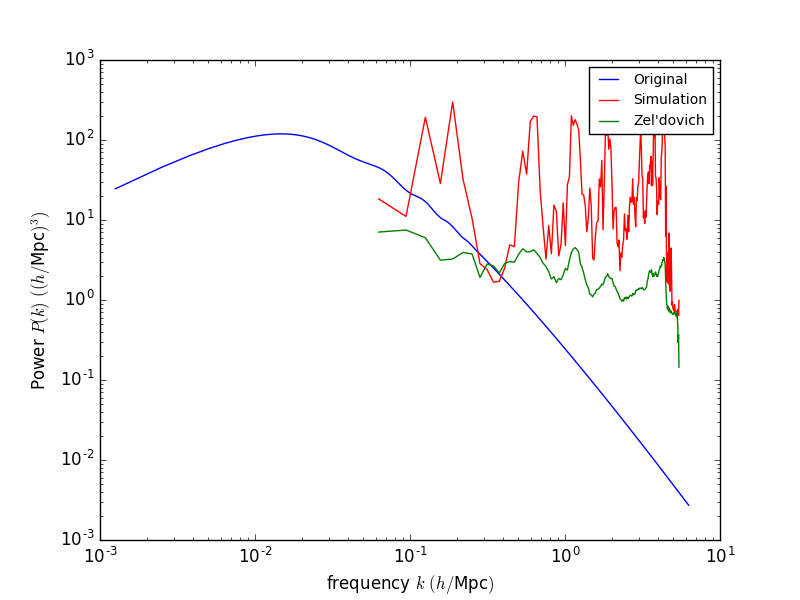
\includegraphics[scale=0.85]{PSComparisonloglog.png}
\caption{Power spectra loglog plots}
\end{figure}

\clearpage

\section*{Analysis}
From Figure 4 we can see that there is significant overlap in the regions of particles in the
simulation results and the Zel'dovich approximation. Additionally, the particles are clustered
more compactly in the simulation results than in the Zel'dovich approximation, as expected. This is due 
to the effects of gravity being present in the simulation and absent from the Zel'dovich approximation.

However, from Figure 5 we can see that there is quite some discrepancy between the original power 
spectrum and the simulated spectra. Although there are some similarities between the simulation power 
spectrum and the Zel'dovich power spectrum, such as the positions of the noise peaks, these are not 
significant There are numerous reasons as to why there is such a difference between the simulated 
and original power spectra.

First and foremost, even though I used a million particles for the simulation, there were only a hundred
particles per dimension. This equates to only a hundred Fourier modes per dimension, which is not
a very large number of data points for a power spectrum, especially when compared to the 5000 in the 
original power spectrum. Further, the first frequency mode of the simulated spectrum
starts at the large value of $0.0628$, which is 50 times $0.00126$, the first frequency in the 
power spectrum used to produce the initial conditions. Therefore, the resolution and frequency range of 
the simulated data was far less than the resolution of the original power spectrum. In order to match the 
resolution, the box size and particle number would have to be increased by a factor of 125,000, which 
would be is incredibly computationally demanding. However, this might be the next order of business, 
so it would be worth finding ways to optimize the code.

This model also assumes that only local forces significantly affects the trajectory of the particle, since 
each adjacent grid point is separated by 1 Mpc/h, a distance at which each particle has a gravitational 
field strength (acceleration field) of $7.0\times 10^{-18}$km/s$^2$ for a simulation of a million particles. 
This is not a very large number, but it certainly adds up for a million particles, especially if some of them
grow very close over time. This conundrum can be handled by using either a better interpolation 
function or a larger range for the cloud-in-cell interpolation.

Finally, the Poisson and gradient solvers use formulas that only apply in the continuous limit. There
are other, more applicable formulas like the Green's function for the discrete case, and it might be
worth using those if sticking to a small number of particles.

All in all, the results look visually correct, as they match the Zel'dovich approximation quite well and
show expected structure.

\end{document}